\section{LENA screen shots}

In this section we show screen shots from the system running several
different image processing algorithms. The image used for the examples
is shown in Figure \ref{fig:lenna_unprocessed}. This figure shows a
screen shot when the system runs a simple \emph{show image/video}
program.

Figure \ref{fig:lenna_negated} shows the image after it has had its
colors negated by a program. Figure \ref{fig:lenna_embossed} shows the
image after being run through an embossing algorithm. In Figure
\ref{fig:lenna_edge_detected}, the image has been run through an edge
detection filter.

The images in these examples have all been processed by the cores in the
SIMD array.

\begin{figure}[h]
  \centering
  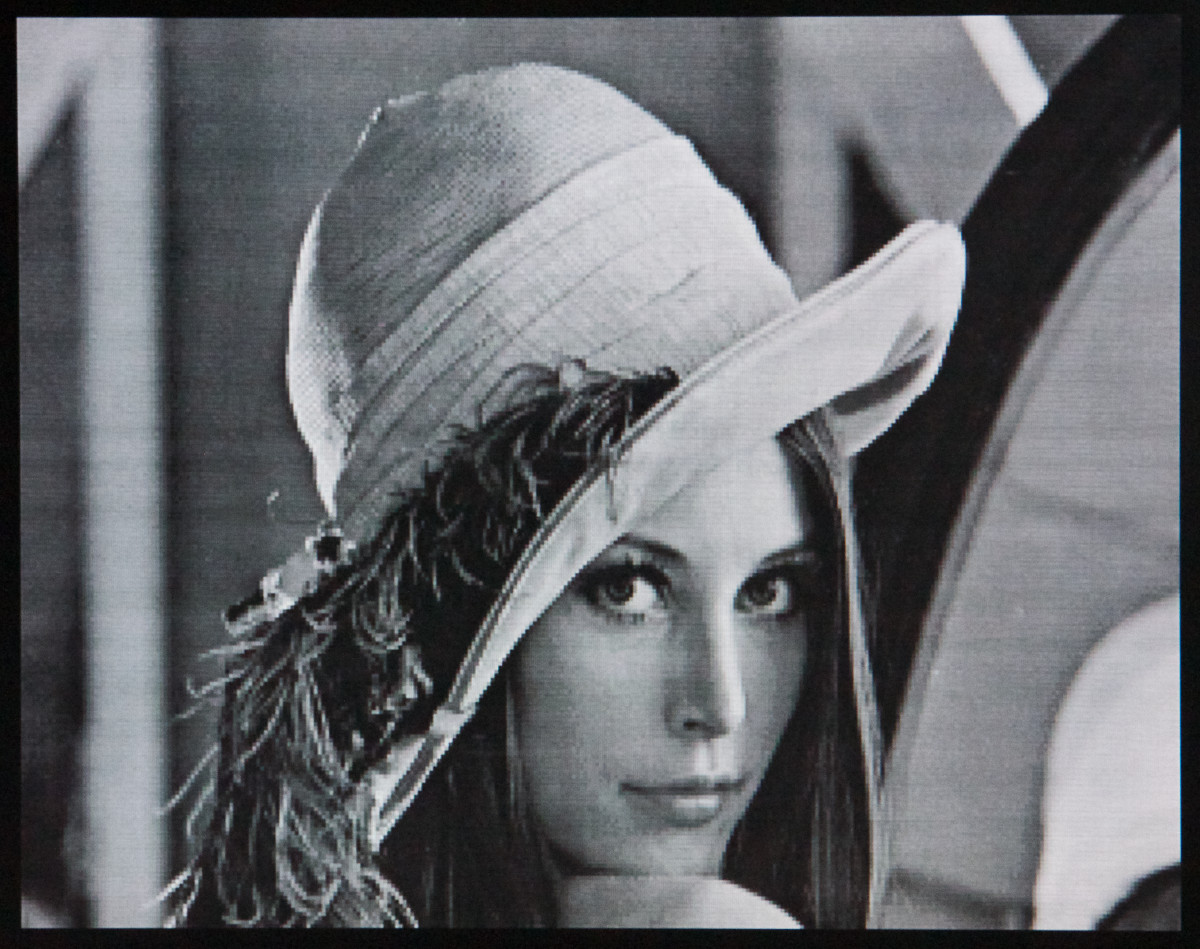
\includegraphics[width=0.8\textwidth]{gfx/results/lenna_unprocessed}
  \caption{Unprocessed image.}
  \label{fig:lenna_unprocessed}
\end{figure}

\begin{figure}[h]
  \centering
  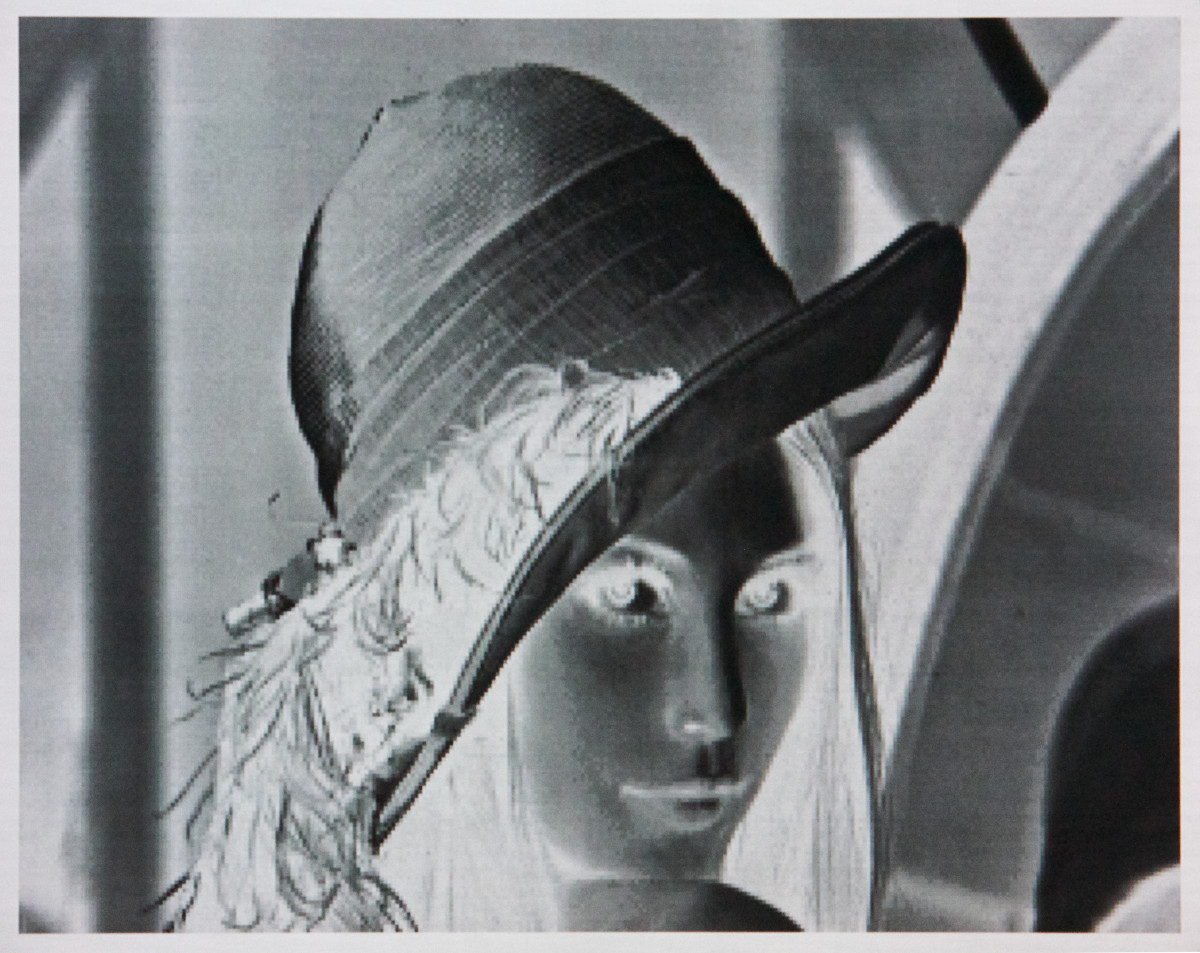
\includegraphics[width=0.8\textwidth]{gfx/results/lenna_negated}
  \caption{Negated image.}
  \label{fig:lenna_negated}
\end{figure}

\begin{figure}[h]
  \centering
  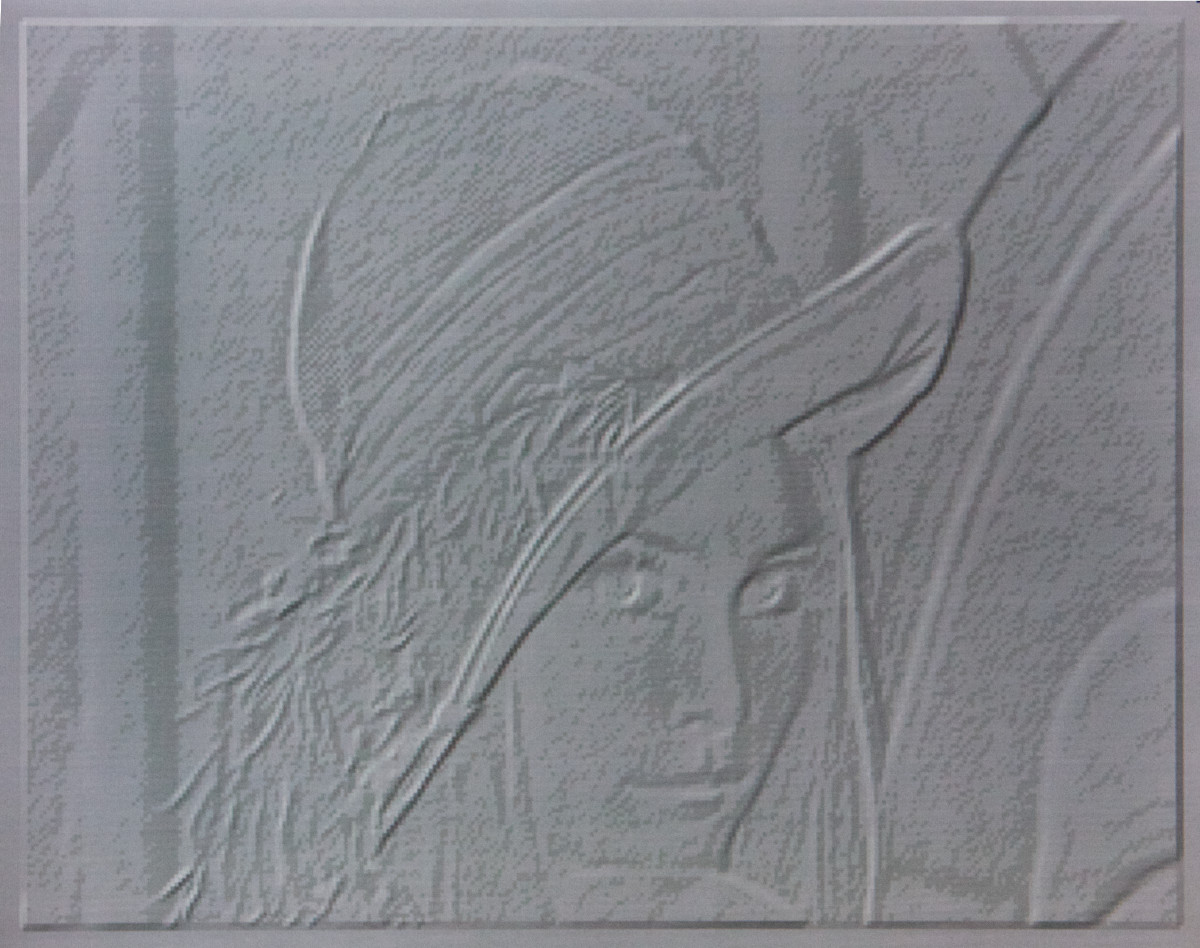
\includegraphics[width=0.8\textwidth]{gfx/results/lenna_embossed}
  \caption{Embossed image.}
  \label{fig:lenna_embossed}
\end{figure}

\begin{figure}[h]
  \centering
  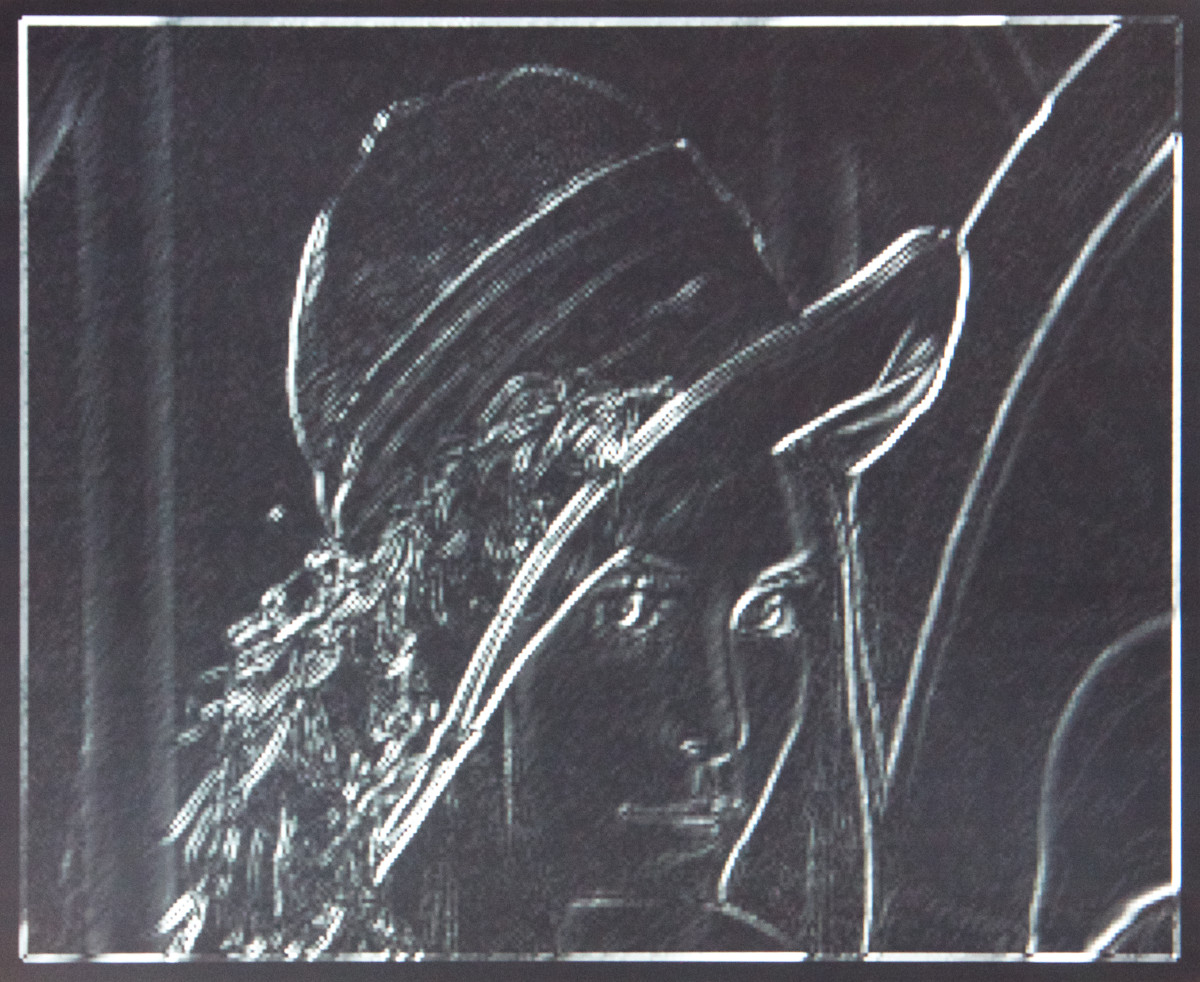
\includegraphics[width=0.8\textwidth]{gfx/results/lenna_edge_detected}
  \caption{Edge detected image.}
  \label{fig:lenna_edge_detected}
\end{figure}
